\chapter{Einleitung}
\label{chap:einleitung}

In dieser Arbeit soll, mit Hilfe einer Simulation, untersucht werden, wie gut sich Kameras bei der Standortbestimmung in mobilen Roboter einsetzten lassen. Anlass dieser Arbeit war eine Anfrage der K�nstlergruppe \ac{BBM}, die schon bei mehreren Performances\footnote{unter Anderem:
  
  2000 Themenpark "Wissen" der Expo 2000 Hannover
  
  2010 Joybots  in der BMW-Welt 
  
  2012 EPKOT Experimental Prototype Killers of Tomorrow , Hannover
  
  siehe auch \url{ http://www.bbm.cfnt3.de}} mobile Roboter eingesetzt haben. Dabei interessierten sie sich f�r eine Lokalisierungsl�sung welche m�glichst ohne weitere spezial Hardware und geringem Installationsaufwand vor Ort auskommt. Der Ansatz der daraus entstand war: die Kameras, die bereits an jedem der Roboter verbaut waren, zu nutzen um markante Muster in der B�hneninstallation zu erkennen und gemeinsam mit den Odometrie-Daten zur Positionsberechnung zu verwenden. Dabei sollte ein Partikelfilter als Zustandssch�tzer verwendet werden. Zu der B�hneninstallation geh�ren gro�e Lichtw�nde, zu sehen auf Abbildung \ref{fig:RobotAndGuests} und \ref{fig:RobotAndLightwall}. Auf diese Lichtw�nde k�nnte ein hell/dunkel Bit-Muster angezeigt werden das es mit Hilfe geeigneter Bildverarbeitungsalgorithmen und mit den Kameras zu erkennen gilt.

  \begin{figure}[p]
    \centering
    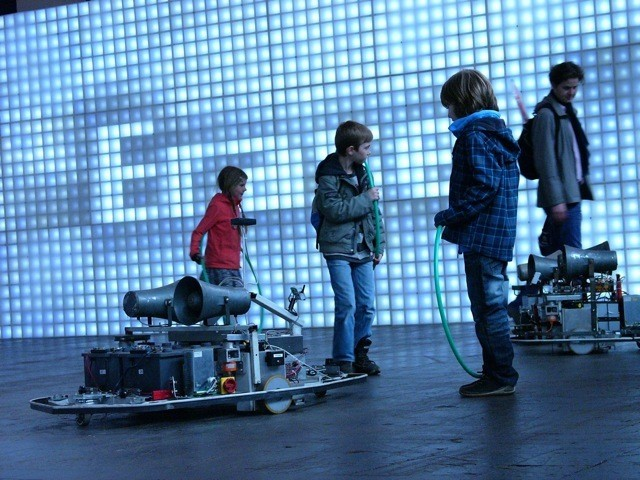
\includegraphics[width=\textwidth]{chapter1/roboterAndLightwallOnEPKOT2.png}
    \caption[Roboter und Besucher auf der EPKOT]{Roboter und Besucher auf der EPKOT Quelle: http://www.bbm.cfnt3.de}
    \label{fig:RobotAndGuests}
    \bigskip 
    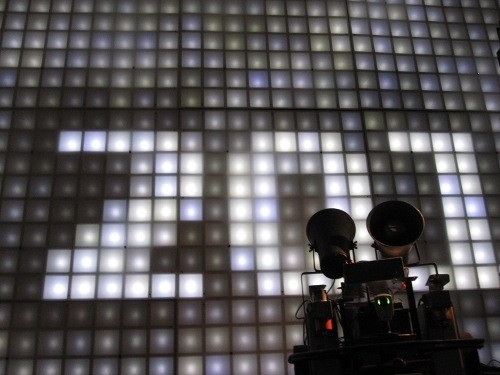
\includegraphics[width=\textwidth]{chapter1/roboterAndLightwallOnEPKOT.png}
    \caption[Roboter vor Lichtwand auf der EPKOT]{Roboter vor Lichtwand auf der EPKOT Quelle: http://www.bbm.cfnt3.de}
    \label{fig:RobotAndLightwall}
  \end{figure}
  
  \section{Ziel und Aufgabenstellung der Arbeit}
Im Rahmen dieser Arbeit soll eine Simulationsumgebung mit Hilfe geeigneter 3D-Visualisierungs Bibliotheken erstellt werden. Die in der Lage ist eine 3D-Szene der B�hne zu simulieren und Kamerabilder sowie Odometrie-Daten einer Roboterfahrt zu erzeugen. Au�erdem soll ein Lokalisationsalgorithmus entwickelt werden, der auf Grundlage dieser Daten die Position und Orientierung des Roboters auf der B�hne sch�tzen kann. Anschlie�end soll die Qualit�t dieser gesch�tzten Position beurteilt werden und m�gliche Fehlerquellen diskutiert werden.

  \section{Gliederung}
Die Arbeit wird im folgenden Kapitel eine kurze �bersicht g�ngiger Lokalisationsverfahren sowie ihre Vor- und Nachteile geben. Au�erdem wird in die Grundlagen eingef�hrt, welche zum Verst�ndnis der folgenden Kapitel notwendig sind. Das Kapitel \textit{\nameref{chap:lokalisierungmittelsbildverarbeitung}} beschreibt wie die Methoden aus den Grundlagen an das gestellte Problem angepasst wurden und wie das vorgestellte Verfahren funktioniert. Anschlie�end wird die Simulations- und Lokalisationssoftware vorgestellt und deren Implementation erkl�rt und begr�ndet. Insbesondere wird darauf eingegangen, wie realistisch die Simulation ist. In Kapitel \ref{chap:versuchsdurchfhrung} beginnt die Beschreibung verschiedener Versuche die zum Beurteilen der Lokalisationsergebnisse durchgef�hrt wurden. Ergebnispr�sentation und Diskussion erfolgen jeweils im Anschluss der Beschreibungen. Abschlie�end wird ein Ausblick zur m�glichen Anwendung dieses Verfahrens gegeben, sowie m�gliche Fehlerquellen und Probleme dabei. Im letzten Kapitel wird ein Fazit zu den Erkenntnissen dieser Arbeit gezogen.
\begin{figure}[htbp]
    \centering
    % GNUPLOT: LaTeX picture with Postscript
\begingroup
  \makeatletter
  \providecommand\color[2][]{%
    \GenericError{(gnuplot) \space\space\space\@spaces}{%
      Package color not loaded in conjunction with
      terminal option `colourtext'%
    }{See the gnuplot documentation for explanation.%
    }{Either use 'blacktext' in gnuplot or load the package
      color.sty in LaTeX.}%
    \renewcommand\color[2][]{}%
  }%
  \providecommand\includegraphics[2][]{%
    \GenericError{(gnuplot) \space\space\space\@spaces}{%
      Package graphicx or graphics not loaded%
    }{See the gnuplot documentation for explanation.%
    }{The gnuplot epslatex terminal needs graphicx.sty or graphics.sty.}%
    \renewcommand\includegraphics[2][]{}%
  }%
  \providecommand\rotatebox[2]{#2}%
  \@ifundefined{ifGPcolor}{%
    \newif\ifGPcolor
    \GPcolortrue
  }{}%
  \@ifundefined{ifGPblacktext}{%
    \newif\ifGPblacktext
    \GPblacktexttrue
  }{}%
  % define a \g@addto@macro without @ in the name:
  \let\gplgaddtomacro\g@addto@macro
  % define empty templates for all commands taking text:
  \gdef\gplbacktext{}%
  \gdef\gplfronttext{}%
  \makeatother
  \ifGPblacktext
    % no textcolor at all
    \def\colorrgb#1{}%
    \def\colorgray#1{}%
  \else
    % gray or color?
    \ifGPcolor
      \def\colorrgb#1{\color[rgb]{#1}}%
      \def\colorgray#1{\color[gray]{#1}}%
      \expandafter\def\csname LTw\endcsname{\color{white}}%
      \expandafter\def\csname LTb\endcsname{\color{black}}%
      \expandafter\def\csname LTa\endcsname{\color{black}}%
      \expandafter\def\csname LT0\endcsname{\color[rgb]{1,0,0}}%
      \expandafter\def\csname LT1\endcsname{\color[rgb]{0,1,0}}%
      \expandafter\def\csname LT2\endcsname{\color[rgb]{0,0,1}}%
      \expandafter\def\csname LT3\endcsname{\color[rgb]{1,0,1}}%
      \expandafter\def\csname LT4\endcsname{\color[rgb]{0,1,1}}%
      \expandafter\def\csname LT5\endcsname{\color[rgb]{1,1,0}}%
      \expandafter\def\csname LT6\endcsname{\color[rgb]{0,0,0}}%
      \expandafter\def\csname LT7\endcsname{\color[rgb]{1,0.3,0}}%
      \expandafter\def\csname LT8\endcsname{\color[rgb]{0.5,0.5,0.5}}%
    \else
      % gray
      \def\colorrgb#1{\color{black}}%
      \def\colorgray#1{\color[gray]{#1}}%
      \expandafter\def\csname LTw\endcsname{\color{white}}%
      \expandafter\def\csname LTb\endcsname{\color{black}}%
      \expandafter\def\csname LTa\endcsname{\color{black}}%
      \expandafter\def\csname LT0\endcsname{\color{black}}%
      \expandafter\def\csname LT1\endcsname{\color{black}}%
      \expandafter\def\csname LT2\endcsname{\color{black}}%
      \expandafter\def\csname LT3\endcsname{\color{black}}%
      \expandafter\def\csname LT4\endcsname{\color{black}}%
      \expandafter\def\csname LT5\endcsname{\color{black}}%
      \expandafter\def\csname LT6\endcsname{\color{black}}%
      \expandafter\def\csname LT7\endcsname{\color{black}}%
      \expandafter\def\csname LT8\endcsname{\color{black}}%
    \fi
  \fi
  \setlength{\unitlength}{0.0500bp}%
  \begin{picture}(8640.00,7200.00)%
    \gplgaddtomacro\gplbacktext{%
      \csname LTb\endcsname%
      \put(1611,2478){\makebox(0,0)[r]{\strut{}-6}}%
      \csname LTb\endcsname%
      \put(1611,4150){\makebox(0,0)[r]{\strut{} 0}}%
      \csname LTb\endcsname%
      \put(1611,5821){\makebox(0,0)[r]{\strut{} 6}}%
      \csname LTb\endcsname%
      \put(2857,1144){\makebox(0,0){\strut{}-6}}%
      \csname LTb\endcsname%
      \put(4529,1144){\makebox(0,0){\strut{} 0}}%
      \csname LTb\endcsname%
      \put(6200,1144){\makebox(0,0){\strut{} 6}}%
      \csname LTb\endcsname%
      \put(1105,4149){\rotatebox{-270}{\makebox(0,0){\strut{}Y-Achse in Metern}}}%
      \put(4528,814){\makebox(0,0){\strut{}X-Achse in Metern}}%
    }%
    \gplgaddtomacro\gplfronttext{%
      \csname LTb\endcsname%
      \put(3673,393){\makebox(0,0)[r]{\strut{}$3\sigma$}}%
      \csname LTb\endcsname%
      \put(3673,173){\makebox(0,0)[r]{\strut{}Trajektorie des Roboters}}%
      \csname LTb\endcsname%
      \put(7696,393){\makebox(0,0)[r]{\strut{}Filter Sch�tzung}}%
      \csname LTb\endcsname%
      \put(7696,173){\makebox(0,0)[r]{\strut{}Update}}%
    }%
    \gplbacktext
    \put(0,0){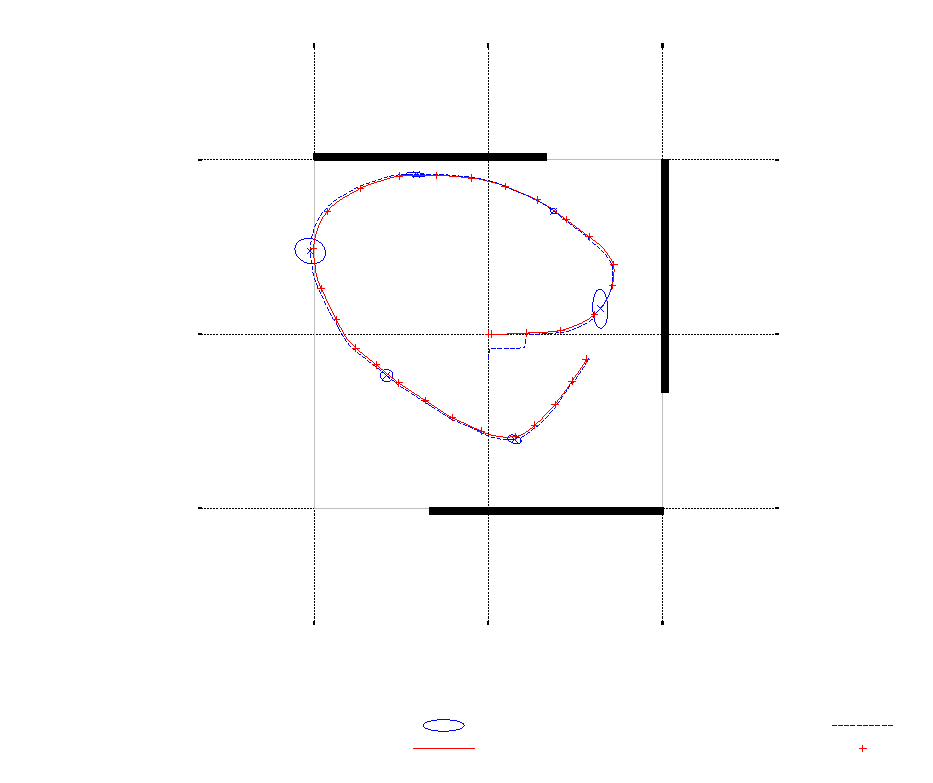
\includegraphics{chapter1/every1000mspics}}%
    \gplfronttext
  \end{picture}%
\endgroup

    \caption{every1000mspics}
    \label{every1000mspics}
\end{figure}
\begin{figure}[htbp]
    \centering
    % GNUPLOT: LaTeX picture with Postscript
\begingroup
  \makeatletter
  \providecommand\color[2][]{%
    \GenericError{(gnuplot) \space\space\space\@spaces}{%
      Package color not loaded in conjunction with
      terminal option `colourtext'%
    }{See the gnuplot documentation for explanation.%
    }{Either use 'blacktext' in gnuplot or load the package
      color.sty in LaTeX.}%
    \renewcommand\color[2][]{}%
  }%
  \providecommand\includegraphics[2][]{%
    \GenericError{(gnuplot) \space\space\space\@spaces}{%
      Package graphicx or graphics not loaded%
    }{See the gnuplot documentation for explanation.%
    }{The gnuplot epslatex terminal needs graphicx.sty or graphics.sty.}%
    \renewcommand\includegraphics[2][]{}%
  }%
  \providecommand\rotatebox[2]{#2}%
  \@ifundefined{ifGPcolor}{%
    \newif\ifGPcolor
    \GPcolortrue
  }{}%
  \@ifundefined{ifGPblacktext}{%
    \newif\ifGPblacktext
    \GPblacktexttrue
  }{}%
  % define a \g@addto@macro without @ in the name:
  \let\gplgaddtomacro\g@addto@macro
  % define empty templates for all commands taking text:
  \gdef\gplbacktext{}%
  \gdef\gplfronttext{}%
  \makeatother
  \ifGPblacktext
    % no textcolor at all
    \def\colorrgb#1{}%
    \def\colorgray#1{}%
  \else
    % gray or color?
    \ifGPcolor
      \def\colorrgb#1{\color[rgb]{#1}}%
      \def\colorgray#1{\color[gray]{#1}}%
      \expandafter\def\csname LTw\endcsname{\color{white}}%
      \expandafter\def\csname LTb\endcsname{\color{black}}%
      \expandafter\def\csname LTa\endcsname{\color{black}}%
      \expandafter\def\csname LT0\endcsname{\color[rgb]{1,0,0}}%
      \expandafter\def\csname LT1\endcsname{\color[rgb]{0,1,0}}%
      \expandafter\def\csname LT2\endcsname{\color[rgb]{0,0,1}}%
      \expandafter\def\csname LT3\endcsname{\color[rgb]{1,0,1}}%
      \expandafter\def\csname LT4\endcsname{\color[rgb]{0,1,1}}%
      \expandafter\def\csname LT5\endcsname{\color[rgb]{1,1,0}}%
      \expandafter\def\csname LT6\endcsname{\color[rgb]{0,0,0}}%
      \expandafter\def\csname LT7\endcsname{\color[rgb]{1,0.3,0}}%
      \expandafter\def\csname LT8\endcsname{\color[rgb]{0.5,0.5,0.5}}%
    \else
      % gray
      \def\colorrgb#1{\color{black}}%
      \def\colorgray#1{\color[gray]{#1}}%
      \expandafter\def\csname LTw\endcsname{\color{white}}%
      \expandafter\def\csname LTb\endcsname{\color{black}}%
      \expandafter\def\csname LTa\endcsname{\color{black}}%
      \expandafter\def\csname LT0\endcsname{\color{black}}%
      \expandafter\def\csname LT1\endcsname{\color{black}}%
      \expandafter\def\csname LT2\endcsname{\color{black}}%
      \expandafter\def\csname LT3\endcsname{\color{black}}%
      \expandafter\def\csname LT4\endcsname{\color{black}}%
      \expandafter\def\csname LT5\endcsname{\color{black}}%
      \expandafter\def\csname LT6\endcsname{\color{black}}%
      \expandafter\def\csname LT7\endcsname{\color{black}}%
      \expandafter\def\csname LT8\endcsname{\color{black}}%
    \fi
  \fi
  \setlength{\unitlength}{0.0500bp}%
  \begin{picture}(8640.00,7200.00)%
    \gplgaddtomacro\gplbacktext{%
      \csname LTb\endcsname%
      \put(1611,2478){\makebox(0,0)[r]{\strut{}-6}}%
      \csname LTb\endcsname%
      \put(1611,4150){\makebox(0,0)[r]{\strut{} 0}}%
      \csname LTb\endcsname%
      \put(1611,5821){\makebox(0,0)[r]{\strut{} 6}}%
      \csname LTb\endcsname%
      \put(2857,1144){\makebox(0,0){\strut{}-6}}%
      \csname LTb\endcsname%
      \put(4529,1144){\makebox(0,0){\strut{} 0}}%
      \csname LTb\endcsname%
      \put(6200,1144){\makebox(0,0){\strut{} 6}}%
      \csname LTb\endcsname%
      \put(1105,4149){\rotatebox{-270}{\makebox(0,0){\strut{}Y-Achse in Metern}}}%
      \put(4528,814){\makebox(0,0){\strut{}X-Achse in Metern}}%
    }%
    \gplgaddtomacro\gplfronttext{%
      \csname LTb\endcsname%
      \put(3673,393){\makebox(0,0)[r]{\strut{}$3\sigma$}}%
      \csname LTb\endcsname%
      \put(3673,173){\makebox(0,0)[r]{\strut{}Trajektorie des Roboters}}%
      \csname LTb\endcsname%
      \put(7696,393){\makebox(0,0)[r]{\strut{}Filter Sch�tzung}}%
      \csname LTb\endcsname%
      \put(7696,173){\makebox(0,0)[r]{\strut{}Update}}%
    }%
    \gplbacktext
    \put(0,0){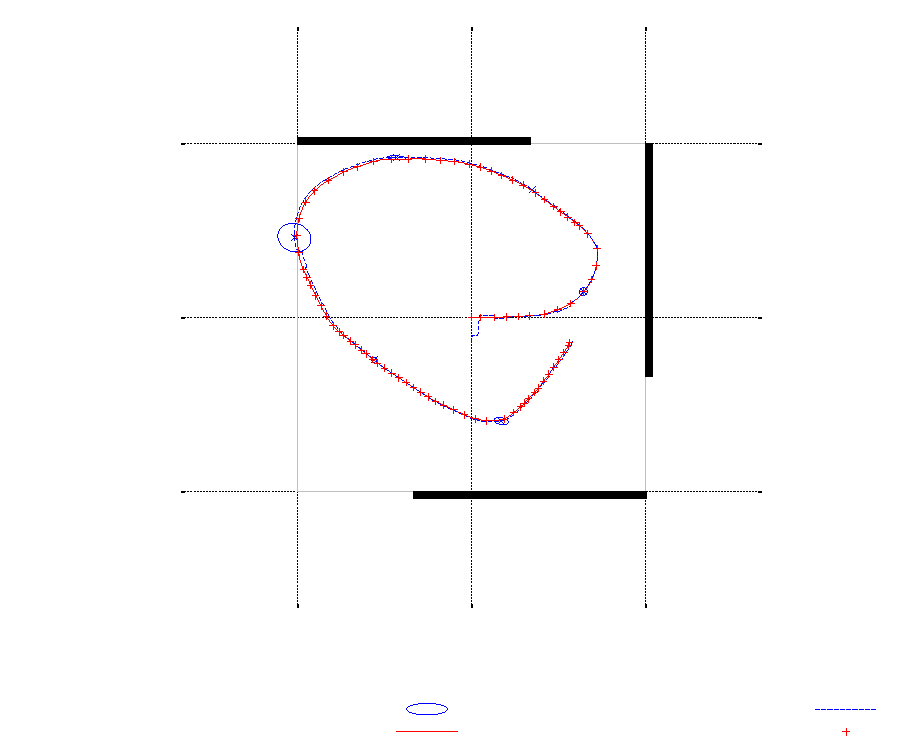
\includegraphics{chapter1/every500mspics}}%
    \gplfronttext
  \end{picture}%
\endgroup

    \caption{every500mspics}	
    \label{every500mspics}
\end{figure}